\documentclass[tikz]{standalone}
\usepackage[utf8x]{inputenc}
\usepackage{tikz}
\begin{document}
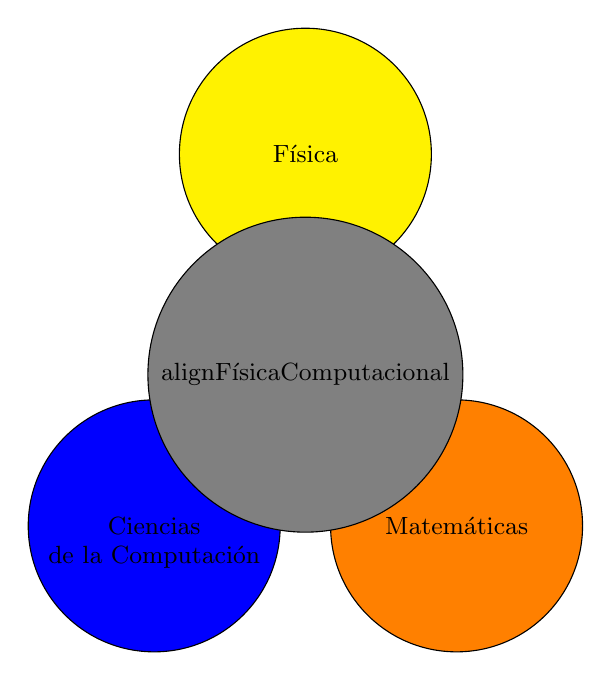
\begin{tikzpicture}[scale=0.8]
%\begin{scope}[fill opacity=0.7]

\draw [fill=yellow, thin] (0,3.5) circle (2);\pause
\draw [font=\small] (0,3.5) node {Física};

\draw [fill=blue, thin] (-2.4,-2.4) circle (2);\pause
\draw [font=\small] (-2.4,-2.4) node {Ciencias};
\draw [font=\small] (-2.4,-2.9) node {de la Computación};

\draw [fill=orange, thin] (2.4,-2.4) circle (2);\pause
\draw [font=\small] (2.4,-2.4) node {Matemáticas};

\draw [fill=gray, thin] (0,0) circle (2.5);\pause
\draw [font=\small align = center] (0,0) node {Física \\ Computacional};
%\end{scope}
\end{tikzpicture}
\end{document}